Following the improvements we have made with the Transaction State
commit mechanism we profiled again YARN. We saw that the performance
was in general better but there were still some cases that should be
improved. These include the time spent when committing a Transaction
State in the database. The actual time required to store some
information to the database was too high. Two cases where examined that
they were slow for two different reasons as explained below.

The first set of operations that where slow to commit were regarding
the RPCs we store for recovery. As I have mentioned earlier Hops-YARN
recovery procedure rebuilds the state of the scheduler from the state
persisted in the database. Moreover, every time the
\emph{ApplicationMasterService} or the \emph{ResourceTrackerService}
receive an RPC they persist it in NDB as well. If the RM crashes, it
will restart or the standby RM will become active, read the latest
RPCs stored in the database and simply replay them. RPCs in the
database are stored in the tables that were depicted in Figure
\ref{fig:impl_fk_yarn_rpc}. We can distinguish between two types of
RPCs. The first type is the heartbeat that the
\emph{ApplicationMaster} sends to the \emph{ApplicationMasterService},
in order to report progress of the application, diagnostics and of
course allocation requests. The second type is the heartbeats that
\emph{NodeManager}s send with the statuses of the containers, health
status of the node etc. Unfortunately, these RPCs can get quite big
in size and considering the limitation of a row size in NDB they had
to be split in multiple tables. For example, if a NM runs 1000
containers then in the heartbeat it will include the status for all of
those. Also, when an AM has just started and makes an allocate
request, this request can contain hundreds of requirements. So the
RPCs are split and stored in the tables as illustrated in Figure
\ref{fig:impl_fk_yarn_rpc}. The \texttt{yarn\_appmaster\_rpc} table
holds general information that is common for both RPCs such as the
\texttt{rpcid} and the \texttt{type} of the RPC whereas the
specific information for allocations or NM status is stored in the
other tables.

The life cycle of an RPC is as follows. First a method is invoked by
an RPC, it decodes the request, which is encoded into a Protocol
Buffers encoding. Then it \textbf{stores} the request in NDB into the
respective tables, it gets the current Transaction State where it adds
the \texttt{rpcid}. Events are triggered, containing the
Transaction State and handled by the RM components. When all the
events have been handled the RPCs that were previously stored are deleted
from the database. If the RM crashes somewhere in the middle, then AMs
and NMs do not have to resend the same information, since RM will read
the last heartbeats from the database. Although, that seems a very
good architecture, persisting and deleting thousands of rows in the
database every second is a tough work and a gain of a few milliseconds
in commit time improves the overall performance.

\begin{figure}
\centering
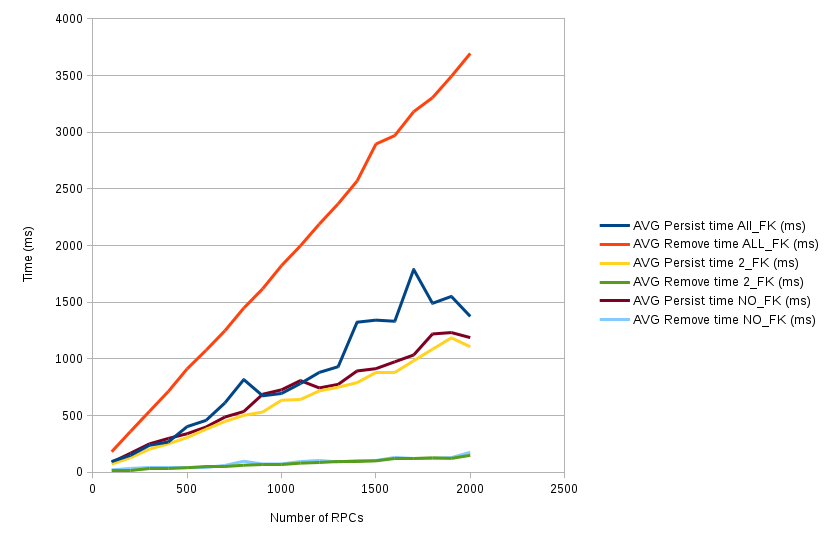
\includegraphics[scale=0.7]{resources/images/Implementation/rpc_fk_overhead.png}
\caption{RPC foreign key constraints micro-benchmark}
\label{fig:impl_fk_overhead}
\end{figure}

If you recall from Section \ref{ssec:impl_fk_appmaster_rpc}, we have
not removed the foreign key constraints from the database schema for
these tables. At that point we discovered that the foreign
key constraints in the RPCs tables really killed performance. I run
some micro-benchmarks to prove the overhead and the results are shown in
Figure \ref{fig:impl_fk_overhead}. The red line in the diagram is the
time needed to remove rows from the tables in Figure
\ref{fig:impl_fk_yarn_rpc}. Then I have changed the schema and removed
the foreign keys. The time to remove the RPCs from the database
without foreign keys is illustrated with the light blue colour. The impact
on performance of foreign keys in our schema was huge. The performance
for persisting data with (blue line) and without (brown) foreign keys
is comparable until 1500 RPCs but then the schema without the foreign
keys performed better. It was clear from the micro-benchmark that
foreign keys should be removed from this set of tables as well. Before
removing completely the constraints we have experimented with a tree
structure of the foreign keys as in Figure
\ref{fig:impl_fk_alternate_schema}. In this schema, only the tables
\texttt{yarn\_heartbeat\_rpc} and \texttt{yarn\_allocate\_rpc} would
have foreign keys to \texttt{yarn\_appmaster\_rpc}. The
micro-benchmark has shown that a schema with two foreign key
constraints has similar performance with a no foreign key constraints
schema. Then the tables specific to AM \emph{allocate} and NM
\emph{heartbeat} would have foreign keys to
\texttt{yarn\_allocate\_rpc} and \texttt{yarn\_heartbeat\_rpc}
respectively. The problem with this setup was the five child tables
of the \texttt{yarn\_allocate\_rpc} table. Considering the overhead of
five foreign keys we have concluded
to remove all the constraints from these tables and implement the
service described in the rest of this section.

\begin{figure}
\centering
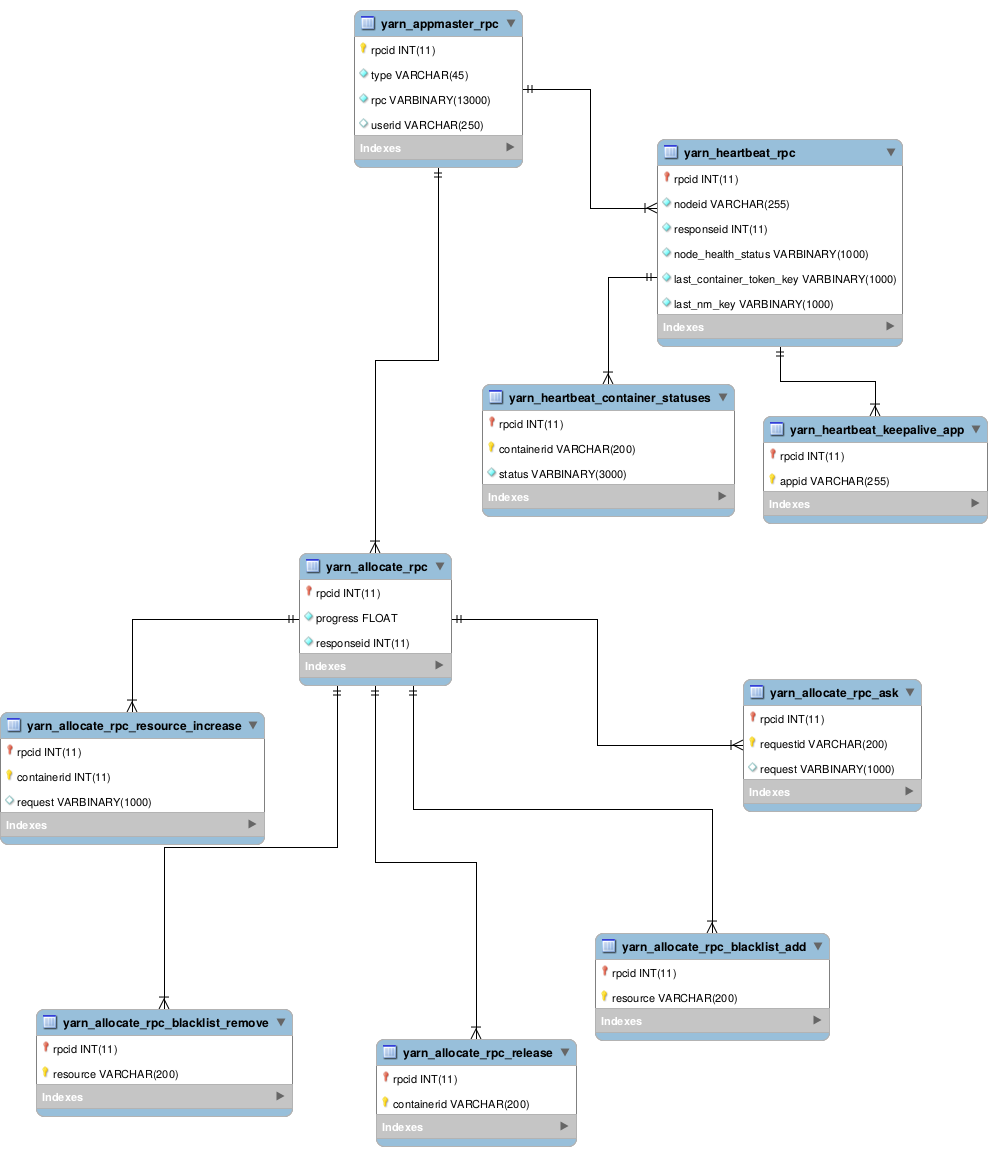
\includegraphics[scale=0.3]{resources/images/Implementation/rpc_fk_alternate_schema.png}
\caption{RPC alternative schema}
\label{fig:impl_fk_alternate_schema}
\end{figure}

The removal of the previously persisted RPCs is part of the
transaction that commits scheduling decisions in the database. If we
are slow in this part, this will increment the commit time of the
whole Transaction State which would make other Transaction States to
be blocked more time in the wait queue having a direct impact on the
cluster utilization. Persisting new RPCs is done when an RPC arrives
and does not directly affect the Transaction State commit time. When
the RM recovers from a failure, it goes through the
\texttt{yarn\_appmaster\_rpc} table and reconstructs the stored RPCs.

In the new implementation, we have created an extra table in the
database called \texttt{yarn\_rpc\_gc} which stores the \texttt{rpcid}
and the \texttt{type} of an RPC. The type can be either
\texttt{HEARTBEAT} or \texttt{ALLOCATE}. When an RPC arrives and
invokes a method, this method will get the Transaction State from the
Transaction State Manager. We add the \texttt{rpcid} and the
\texttt{type} of that RPC in the data structures of the TS and are
persisted in the database. When all of the RPCs have been handled
properly, at the same transaction, \textbf{only} the rows from
the \texttt{yarn\_appmaster\_rpc} table are removed and \textbf{not}
from the others, opposed to the previous solution. The entries at the other tables are taken care by the
\emph{Garbage Collector} service.

\emph{Garbage Collector} (GC) is a Hops-YARN service that purges
asynchronously old RPC entries from the database. The main thread of
GC reads the \texttt{rpcid}s and \texttt{type}s from the
\texttt{yarn\_rpc\_gc} table. Then it creates a number of threads that
will delete the rows with a specific \texttt{rpcid} from all the other
tables. The threads will create
queries that will remove the rows where the column \texttt{rpcid}
equals the specific \texttt{rpcid} fetched by the
\texttt{yarn\_rpc\_gc} table. The tables affected for the AMs'
allocate RPCs are:
\begin{itemize}
\item \texttt{yarn\_allocate\_rpc}
\item \texttt{yarn\_allocate\_rpc\_ask}
\item \texttt{yarn\_allocate\_rpc\_blacklist\_add}
\item \texttt{yarn\_allocate\_rpc\_blacklist\_remove}
\item \texttt{yarn\_allocate\_rpc\_release}
\item \texttt{yarn\_allocate\_rpc\_resource\_increase}
\end{itemize}

The rows for the NMs' heartbeats are removed from the tables:
\begin{itemize}
\item \texttt{yarn\_heartbeat\_rpc}
\item \texttt{yarn\_heartbeat\_container\_statuses}
\item \texttt{yarn\_heartbeat\_keepalive\_app}
\end{itemize}

The only performance drawback that we have with the GC service is that
the deletion queries do not operate on primary keys. There is a
trade-off here. The current implementation uses only one table for the
RPCs to be removed that store the \texttt{rpcid} and the
\texttt{type}. For that reason we cannot do primary key operations but
we persist less data in the Transaction State. Since, the removal of
the RPCs is done asynchronously it does not affect the commit time
of the TS. Also, the \texttt{rpcid} in the RPC tables is indexed so we
do not perform a full table scan and is also the partition key so we avoid RTT
among NDB Data Nodes. The other alternative would be to
store all the necessary information to build the primary keys for the
rows to remove. This would effectively mean that we would need to persist more
data during the commit of the TS that might increase the commit
time. Also, we should have had more than one table to store them,
making the schema more complex. Since the Active RM -- scheduler is
already overloaded with making scheduling decisions, handling AM
heartbeats, etc we decided that the Garbage Collector service will run on
the leader of the standby RMs -- ResourceTrackers.

The asynchronous removal of entries from NDB off-loaded the Transaction
State commit phase in that extend that we decided to use it also for
another case that it took more time to persist data than that we
desired. That is the case of Allocate Response. When the AM registers
with the RM or when it requests resources on the cluster, the
scheduler generates an allocate response that is sent back to the
AM. This allocate response is persisted in the database through the
Transaction State for recovery reasons. In some cases it can contain a
lot of information for example when the AM registers and requests all
of its requirements. When the scheduling decision is made, the scheduler creates a response with the
containers requested. The tables used in the database to store such
allocate response are: \texttt{yarn\_allocate\_response},
\texttt{yarn\_allocated\_containers} and
\texttt{yarn\_completed\_containers\_statuses}. The main problem in
that case was that when we were persisting an allocate response, first we
had to delete the previous response generated by the
scheduler. So each addition to the database, implicitly means an extra
deletion. The delete operation should remove probably hundreds of
rows of allocated containers and completed containers' status. We
followed the same method as described above with the RPCs. A new table
was put in the schema, \texttt{yarn\_alloc\_resp\_gc}, that is
storing the necessary information for the GC to remove previous
allocation responses. That way, during the commit phase of the
Transaction State we only add new responses and \textbf{not} removing
the old ones, reducing more the commit time of a TS.

Removing entries from the database in an asynchronous way raises some
discussion about the consistency model. For example what will be the
state recovered by the scheduler if old RPCs or allocate responses
have not been deleted yet. Regarding the recovery of RPCs, when the
failed RM tries to construct the last state from the database, it
fetches all the entries stored in the RPC tables and joins the split
parts. The detail that makes the system work is that it consults the
\texttt{yarn\_appmaster\_rpc} table about the \texttt{rpcid}s of the
RPCs that had not been handled when the RM crashed. Since the entries
for that table are removed synchronously in the commit phase of the
Transaction State, we guarantee that this table will not contain any
rubbish. So the RPCs that will be joined and re-constructed will be
real not handled RPCs. The only drawback is that it might take more
time to read the RPC tables since they might contain more rows than
actually needed. In addition, the GC runs on the RT so until the new
RM makes a transition from standby to active and recover the persisted
state, the old RPCs would have been collected. The same philosophy
applies for the Allocate Responses. The old allocate response of an
application is removed synchronously from table
\texttt{yarn\_allocate\_response}, by the Transaction State. Each
response has an incremented ID. At any time, there is only one ID for
each application attempt stored in this table. When the scheduler
constructs the last allocate response before it crashed, it filters
the entries read from \texttt{yarn\_allocated\_containers} and
\texttt{yarn\_completed\_containers\_statuses} with the valid response ID.